\documentclass[12pt]{article}
\usepackage[pdftex]{color, graphicx}
\usepackage{amsmath, amsfonts, amssymb, mathrsfs}
\usepackage{dcolumn}
\usepackage{natbib}
\usepackage{graphicx}
\usepackage{geometry}
\usepackage{listings}
\usepackage{hyperref}

\title{Topics in Biostat Final Report: Use CNN to Predict Stock Returns}
\author{Li Xu}
%\date{Dec.2 2015}

%\geometry{left=2cm,right=2cm,top=1.5cm,bottom=1.5cm}
\begin{document}
\maketitle

\section{Introduction}
In this project, we try to use the price chart of stocks to predict the next day's return. For data collecting, we developed a reliable software to scrap the data from financial website and plot the stock historical chart automatically.  We use con convolutional neural network (CNN) and fully connected neural network to build our deep learning structure. We perform a two stage prediction. One is binary classification that we predict whether the price will increase or decrease. The other is to predict the next-day return of a stock (continues output). 

\section{Data Description and Collecting}
First step of this project is to define our input and output of our model. We wants to use the previous 30 days data of one stock to predict the return on 31 days. Let $P_1$ be the close price on the first day and $P_{31}$ be the close price on 31st day. The return $R$ we want to predict is calculated by:
\begin{align}
R=\frac{P_{31}-P_1}{P_1}
\end{align}

For our input, we wants to use the image. Stock chart is good visualization tools to display the change of history. Since CNN gives us a change to directly use image for input. We use the chart built by 30-days stock price as our model input.  An example stock chart is shown in Figure (\ref{fig:chart}).

We randomly selected 200 stocks from the Standard \& Poor's 500 index(SP500) as our data source. We use the data after 2016-01-01. To get enough data, we further assume the stocks in SP500 are "identical". That means each stocks has similar behavior and they can be combined to build our training set. For example, we have one chart from AAPL and one chart form ABT, they are treated as two points in our training set. In the above assumptions, we totally got \textbf{3250} images.

We use quandl package for retrieving data and plotly for plotting charts. We encounter some issues when scraping data and making plot. If you request data too frequent (for example, use loop to download data), the remote server will refuse your request for a while. So  we set a 3 second pause after we draw each plot.

\begin{figure}[h]
	\centering
	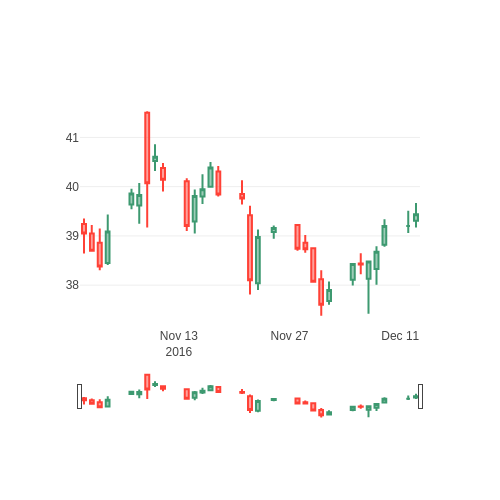
\includegraphics[scale=0.8]{ABT}
	\caption{Example stock chart built from Abbott Laboratories(ABT)'s historical price.}
	\label{fig:chart}
\end{figure}

\section{Data Preprocessing}
Before we train our model, we need to do some data preprocessing. For the resolution of image, we make them to be $500\times500$. We assume all stocks are "identical" so we remove the caption of chart. Another issue is the color of the image. The original image in Figure (\ref{fig:chart}) is colorful. So if you read the image in python, it should be a $(500, 500, 4)$ tensor. This is too big considering we have 3250 images. Converting them to black and white seems we reduce the information too much. The color in image should makes sense. Eventually, we transfer the image to gray scale. One example for same chart before and after gray scaled is provided in Figure (\ref{fig:gray}). The scaled one looks yellow because I did not specify the color space when printing. If you specify the color space to be gray, if should looks normal. After preprocessing, our model input should be a $500\times500$ matrix.

We also split the data into training set and testing set. Since we did not set valid set because our sample size is relatively small. 
\begin{figure}[h]
	\centering
	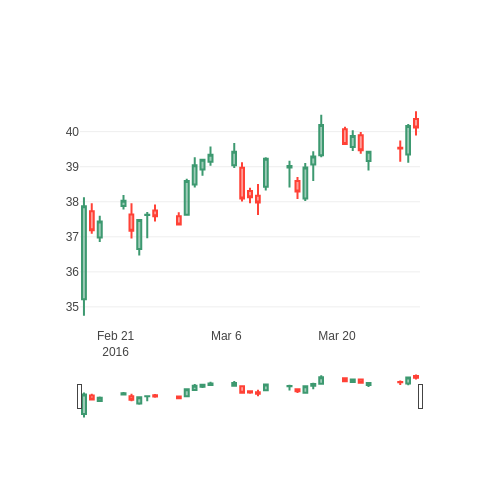
\includegraphics[scale=0.5]{iA}
	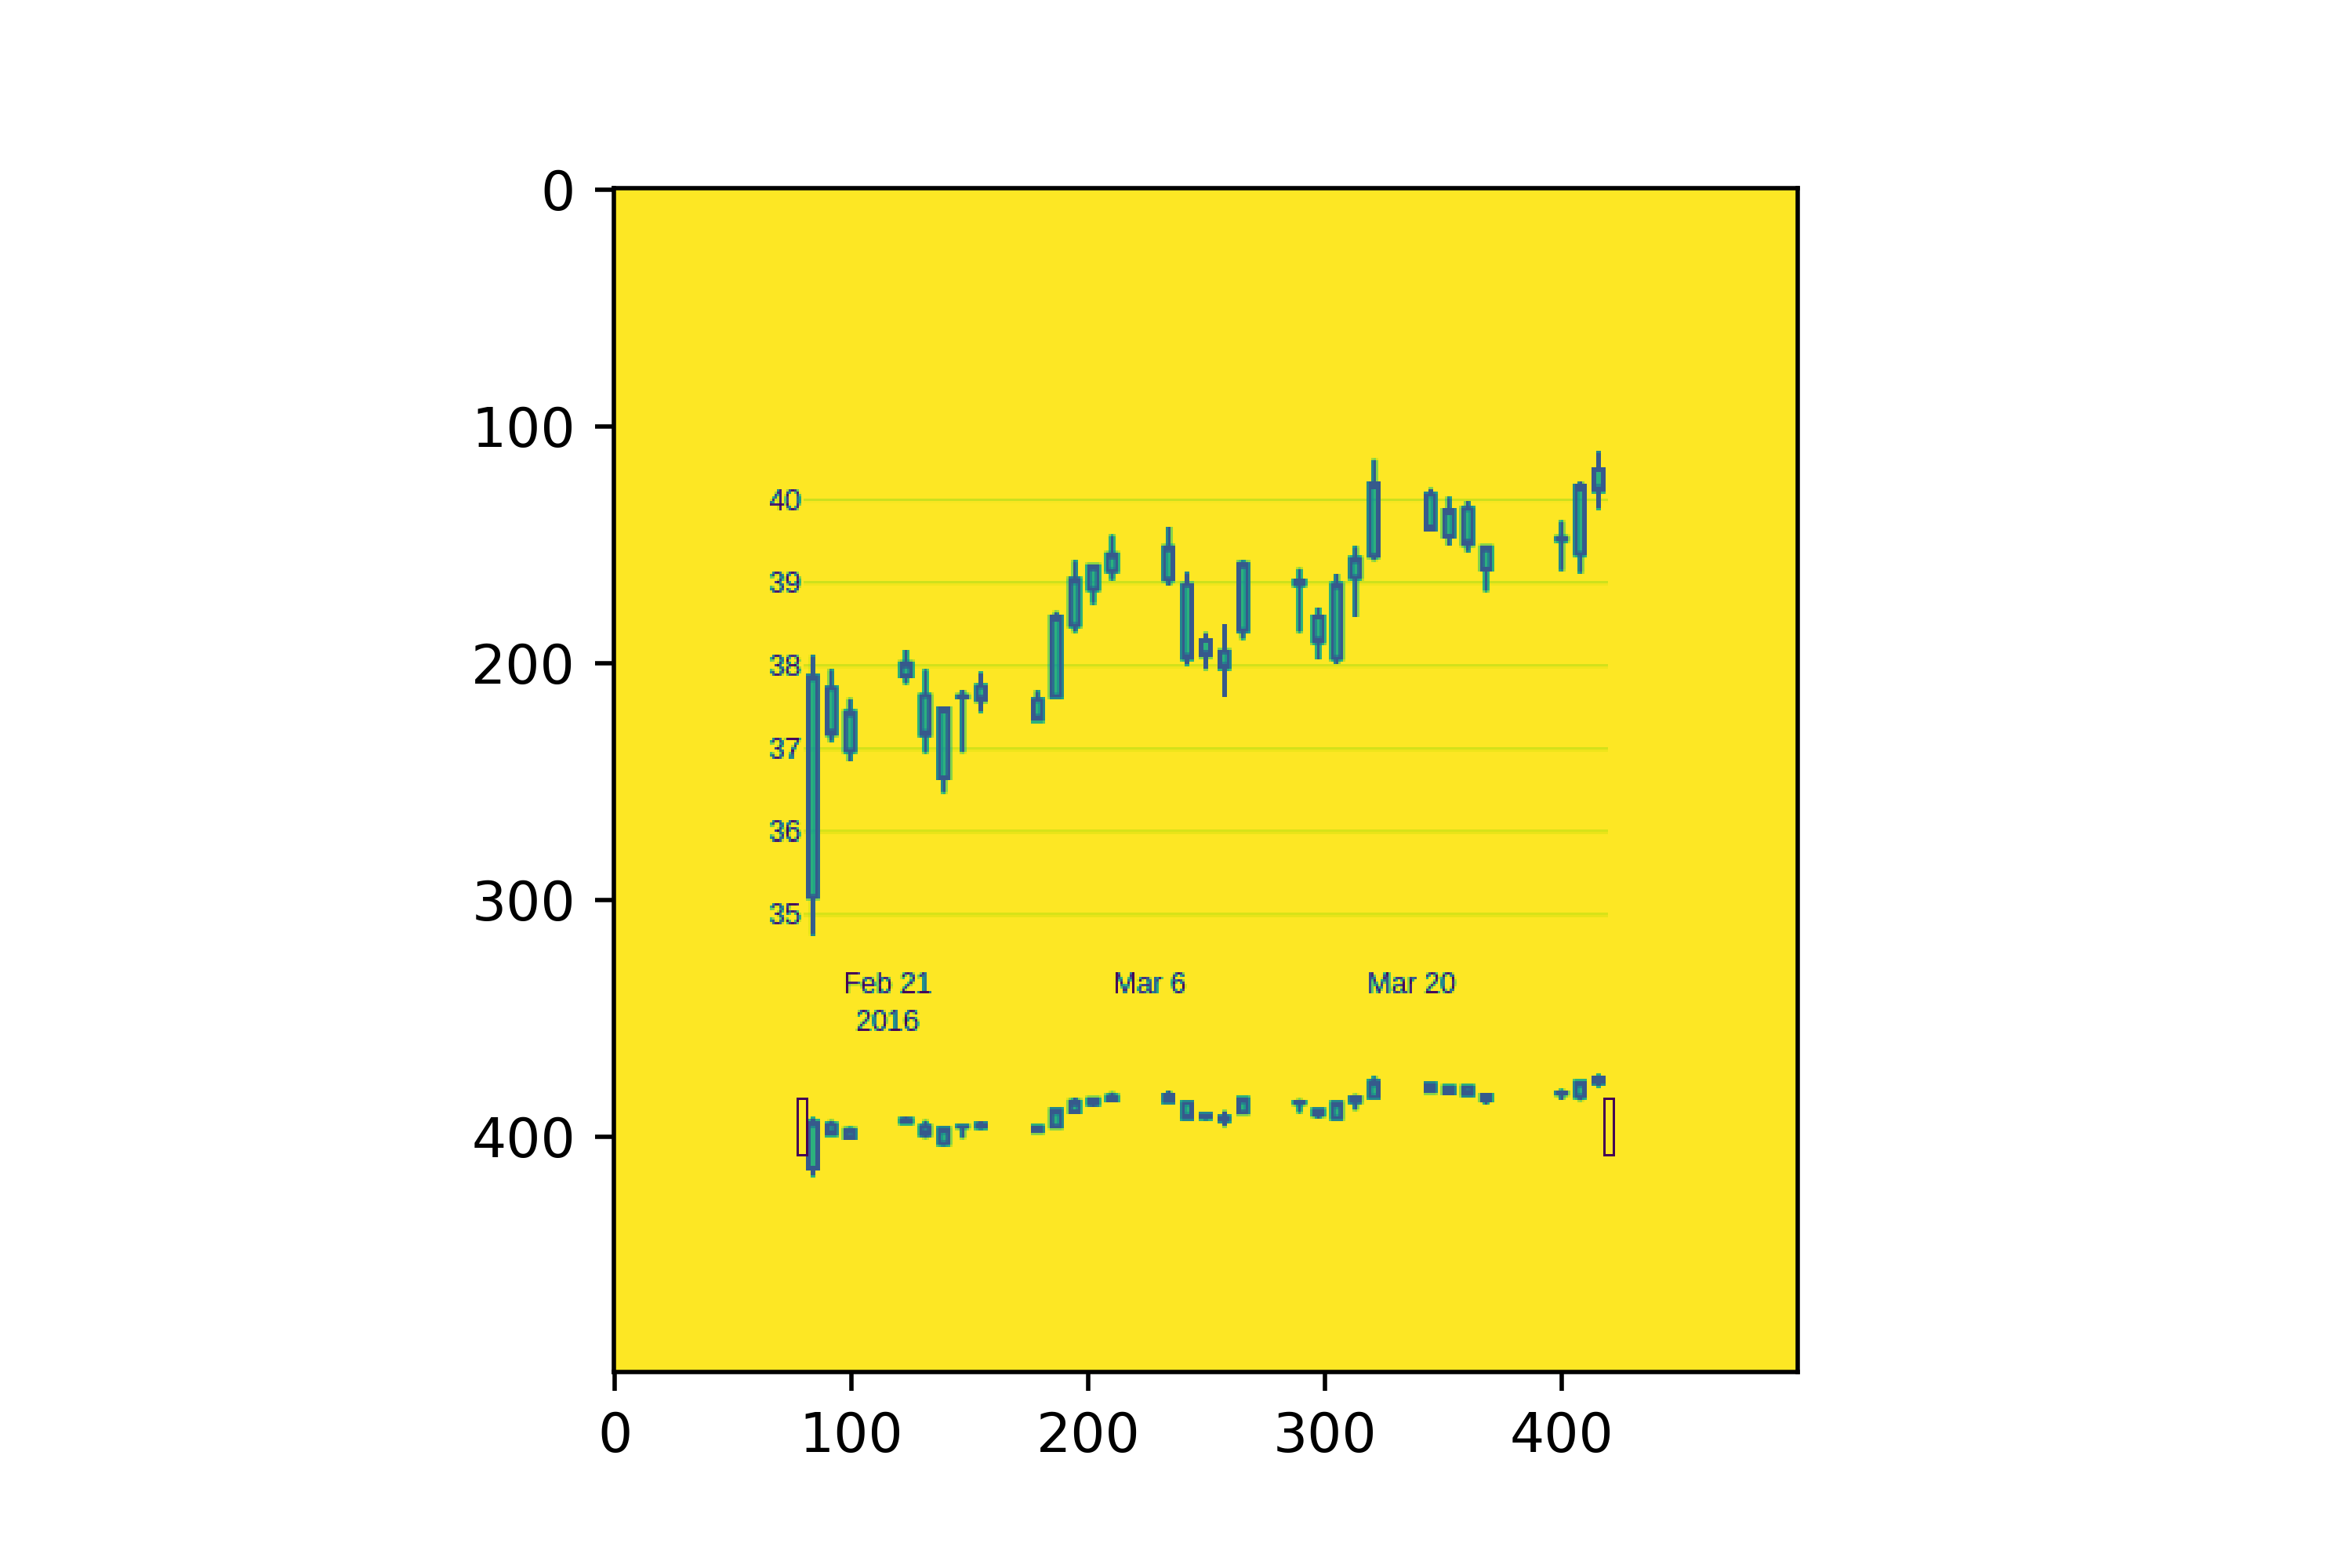
\includegraphics[scale=0.8]{iAgray}
	\caption{Example of Gray Scale, Upper is the original chart and below is the scaled one.}
	\label{fig:gray}
\end{figure}

\section{Deep Learning Neural Network Structure}
\subsection{Binary Prediction}
First we predict given a chart built by the previous 30-day price, whether the stock will increase or decrease. The output is binary and we let "0" means decrease and "1“ means increase.  I use a model with CNN and fully connected layers. The code for build the architecture is in Figure (\ref{fig:m1}). The training output is in Figure (\ref{fig:tr1}) The confusion matrix are also provided in Figure (\ref{fig:cm}). We use categorical hinge for the loss function.

From the confusion matrix, we see that CNN does not have the power to classify the stock increase on our current dataset.
\begin{figure}[h]
	\centering
	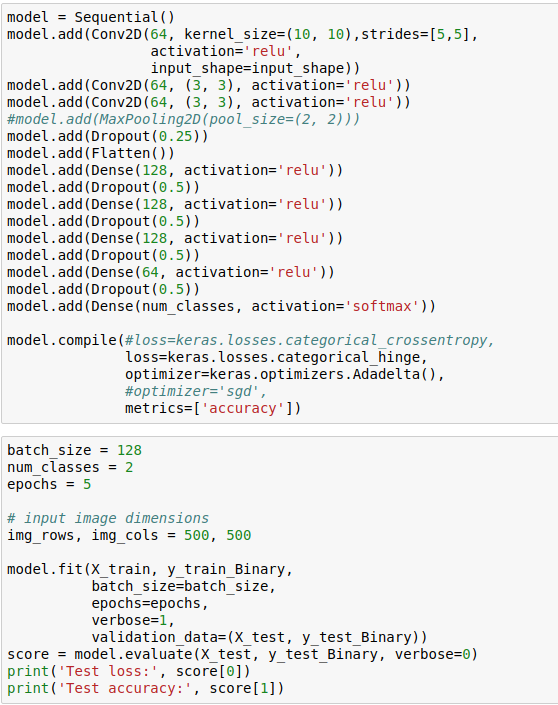
\includegraphics[scale=0.6]{model1}
	\caption{Model code for Binary Output.}
	\label{fig:m1}
\end{figure}

\begin{figure}[h]
	\centering
	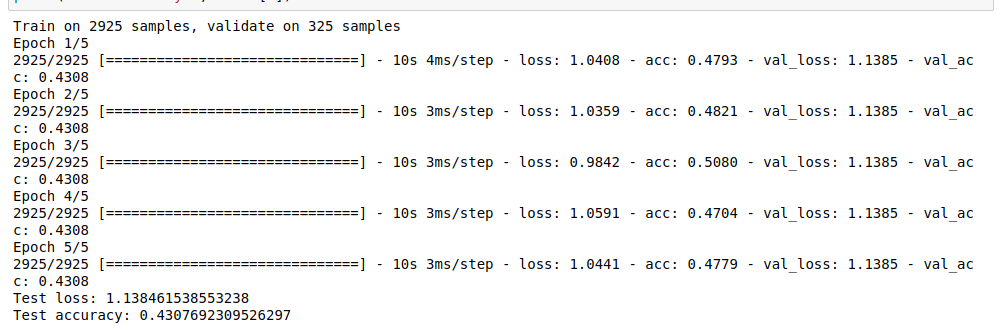
\includegraphics[scale=0.5]{res1}
	\caption{Training Output for Binary Output.}
	\label{fig:tr1}
\end{figure}

\begin{figure}[h]
	\centering
	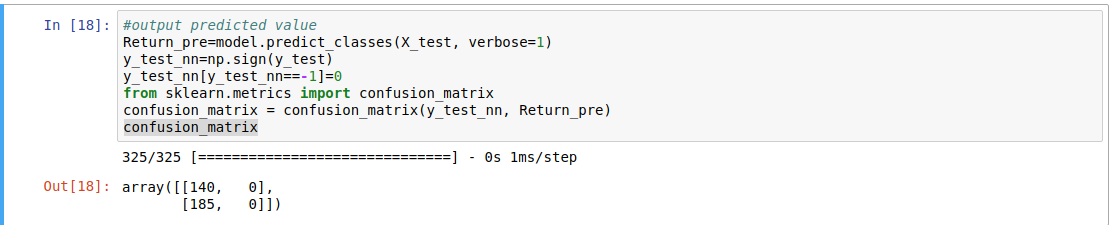
\includegraphics[scale=0.7]{confusionM}
	\caption{Confusion Matrix for Binary Output.}
	\label{fig:cm}
\end{figure}


\subsection{Continues Prediction}
The second stage of our prediction is to predict the stock return on 31st days. We use the same structure in Chapter 3 but change the output layer to be continues output. The model code is in Figure (\ref{fig:m2}). The training output is in Figure (\ref{fig:tr2}). Again, the model fails at predicting the stock price.

\begin{figure}[h]
	\centering
	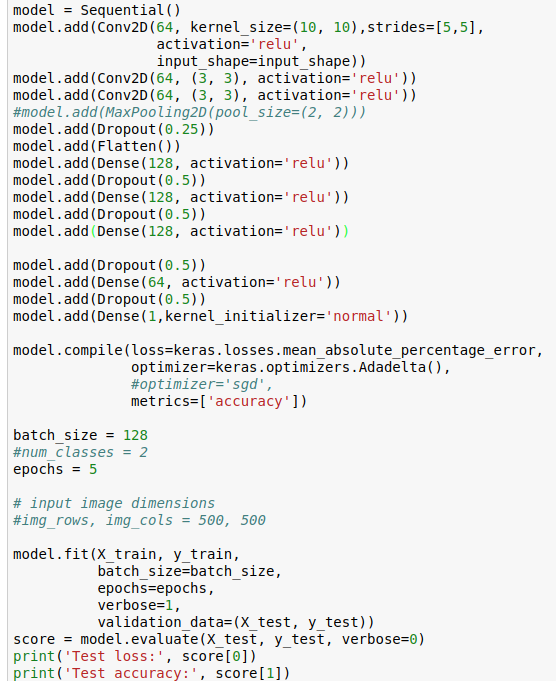
\includegraphics[scale=0.6]{model2}
	\caption{Model code for Continues Output.}
	\label{fig:m2}
\end{figure}

\begin{figure}[h]
	\centering
	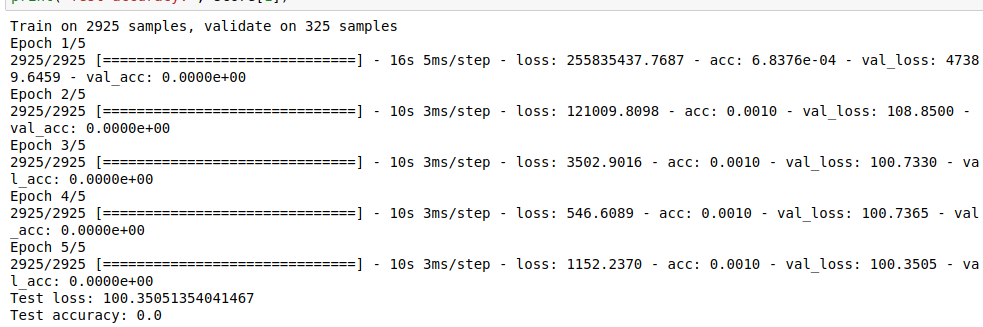
\includegraphics[scale=0.5]{res2}
	\caption{Training Output for Continues Output.}
	\label{fig:tr2}
\end{figure}

\section{Results and Summary}
In this project, we fail to make any meaningful prediction for the stocking price. Some reason may be concluded. First, our training sample is too limited. In the mnist examples. The training set is 60000 which is much larger than ours. Due to the limit time, we are not able to produce more dataset. We must pause between each data requesting to avoid being prohibited for some time due to the API's regulation. This greatly affects our data collecting speed. 

Second, our deep learning structure is too simple. Stocking price is famous for its difficulty to be predicted. So we can image the latent architecture should be complex. Due our limit computing power, we are not able to train more complex model. We use a GTX1070 on my desktop for training and it is easy to get a memory overflow error. 

Last but not lease, we create a framework for doing prediction on stock price. If giving more time, we may get better results. 

\clearpage
\appendix
\section{Repo}
All of our code is available online. The URL for the repo is  \href{https://github.com/tgh1122334/surfdeep/tree/master/finalProj}{here}.
\end{document}